\documentclass[tikz]{standalone}
\usepackage{fontspec}
\renewcommand*{\familydefault}{\sfdefault}
\usepackage{standalone}
\usetikzlibrary{arrows.meta, decorations.pathreplacing, shapes.geometric}
\usetikzlibrary{bayesnet}

\begin{document}

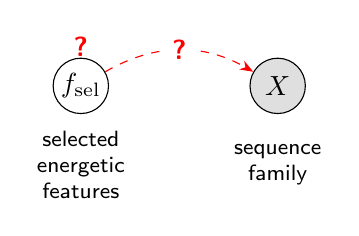
\begin{tikzpicture}
% Define nodes
\path (0,0)
node[obs] (X) {\(X\)}
to
(180:2.5 cm)
node[latent] (fsel) {\(f_\mathrm{sel}\)}
;

\path[font=\footnotesize]
(X) +(-90:1 cm) node[align=center] {sequence\\family}
(fsel) +(-90:1 cm) node[align=center] {selected\\energetic\\features}
;

\begin{scope}[every node/.style={font=\bfseries, text=red}]
\draw[dashed, red, -Stealth]
(fsel) to[bend left] node[fill=white] {?} (X);
\path (fsel) +(90:0.5) node {?};
\end{scope}

\end{tikzpicture}
\end{document}


